
\chapter{Masterframe}
\label{cha:masterframe}

In dit hoofdstuk zal er een masterframe gebouwd worden zoals beschreven in \cite{Tessema}. Voor er hier aan begonnen wordt moet er nagedacht worden over wat de robot allemaal kan en hoe die zou gebruikt kunnen worden door een gebruiker. De robot is te zien in figuur \ref{robot}. Hij kan vooruit en achteruit rijden, hij kan draaien, hij heeft een grijper vooraan waarmee hij dingen kan oppakken en hij heeft een aantal sensoren om objecten te detecteren en om aan tracking te doen. \\

\begin{figure}[h]
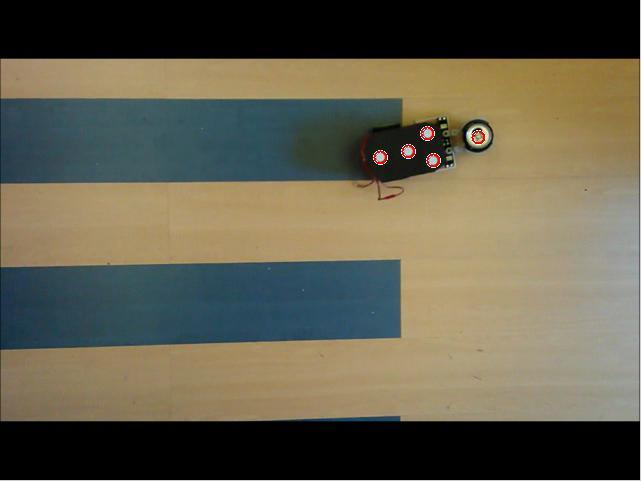
\includegraphics[width=0.5\textwidth]{robot.jpg}
\label{robot}
\centering
\caption{foto van de gebruikte robot}
\end{figure}


De eenvoudigste opdrachten dat een gebruiker de robot zou kunnen geven is om te bewegen. Zaken zoals 'ga naar daar' of  'rij 5cm vooruit' zijn hiervan een voorbeeld. Er wordt hier onderscheid gemaakt tussen drie soorten bewegingen dat een gebruiker zou kunnen vragen van de robot:

\begin{itemize}
\item een absolute beweging: dit is een beweging naar een vast punt in de frame zoals bv. de hoek of het midden. Dit zou ook een object kunnen zijn.
\item een relatieve beweging: dit is een beweging relatief ten opzichte van zijn huidige positie zoals een bepaalde afstand voorruit of naar links rijden. 
\item bewegen voor een bepaalde tijd: dit kan zijn tot de gebruiker stop zegt of voor een bepaalde tijdsspanne.
\end{itemize}

Elke soort van de opgesomde bewegingen kan een rotatie en/of een translatie bevatten.  \\
\\
Andere commando's zijn commando's waarvoor de robot zijn grijper nodig heeft. Dit zouden eenvoudige dingen kunnen zijn zoals 'grijp' of 'laat los'. Voor deze commando's moet de robot maar een actie uitvoeren respectievelijk zijn grijper sluiten of openen. Er zijn echter ook complexere commando's zoals 'breng het blikje naar de bal'. Hiervoor moet de robot verschillende dingen doen; Hij moet het blikje vinden, naar het blikje rijden, het blikje pakken, de bal vinden, naar de bal rijden en zijn grijpers openen.\\
\\
Uit de bovenstaande beschrijving wordt er een lijst van mogelijke commando's gehaald. Deze lijst is te zien in tabel \ref{commands}.

\begin{table}[h]
\centering
\begin{tabular}{| l | l |}
\hline
\textbf{move\_rel} &  bewegen relatief ten opzichte van de huidige positie\\
\textbf{move\_abs} & bewegen naar een vast punt in de frame\\
\textbf{move\_to\_obj} & bewegen naar een object\\
\textbf{move\_time} & bewegen voor een bepaalde tijd\\
\textbf{turn\_abs} & zich richten naar een bepaalde richting\\
\textbf{turn\_rel} & een bepaalde hoek draaien relatief ten opzichte van de huidige ori"entatie\\
\textbf{turn\_time} & draaien voor een bepaalde tijd\\
\textbf{grab} & grijpen met de grijpers\\
\textbf{release} & de grijpers openen\\
\textbf{grab\_obj} & een bepaald object pakken\\
\textbf{move\_obj} & een object verplaatsen naar een andere locatie\\
\textbf{stop} & stop de huidige actie\\
\hline
\end{tabular}
\caption{lijst van commando's}
\label{commands}
\end{table}

Voor alle commando's dat zijn opgesomd in tabel \ref{commands} moet er beslist worden welke waarden er moeten worden meegegeven met de commando's en wat die waarden allemaal zouden kunnen zijn. De commando's zouden op een zo natuurlijk mogelijke manier moeten kunnen gegeven worden. Een normale gebruiker zal bijvoorbeeld zelden zeggen: 'rij naar positie met x-co"ordinaat 3 en y co"ordinaat 5' maar zal eerder iets zeggen als 'rij naar het midden'.\\
\\
Voor de afstanden dat de robot relatief ten opzichte van zijn huidige positie kan afleggen wordt er gekozen voor een exponentieel verloop omdat voor kleine bewegingen van de robot een hogere precisie nodig is als bij grotere bewegingen.\\
De robot kan ook bewegen naar vaste punten. Zoals al vermeld moeten deze punten benoembaar zijn in natuurlijke taal e.g. 'het midden'. Daarom wordt voor de vaste posities gekozen voor het midden, de hoeken en het midden van de wanden. Deze plaatsen zullen benoemd worden zoals de windrichtingen.\\
Voor de acties waarbij de robot moet bewegen voor een bepaalde tijd moeten er verschillende aantallen seconden zijn maar het moet ook mogelijk zijn om de robot te laten bewegen tot de gebruiker stop zegt (de rotatie kan zo bv gebruikt worden om de robot te richten). De tijden worden net als de afstanden exponentieel gekozen.\\
De hoeken dat de robot moet kunnen draien moeten alsook in de natuurlijke taal benoemd kunnen worden. Logische keuze's zijn alvast $90^\circ$ en $180^\circ$ voor bv. 'draai naar links' of 'draai om'  $45^\circ$ is ook nog gekozen voor bv 'draai schuin naar rechts'.\\
Het absoluut richten van de robot moet mogelijk zijn naar alle 'windrichtingen' gekozen voor de absolute bewegingen. De hoeken zijn dus gekozen van $0^\circ$ in stappen van $45^\circ$ tot $315^\circ$.\\
\\
Met al deze gemaakte beslissingen kan nu het masterframe worden opgesteld. Deze is te zien in figuur \ref{masterframe}

\begin{figure}[h]
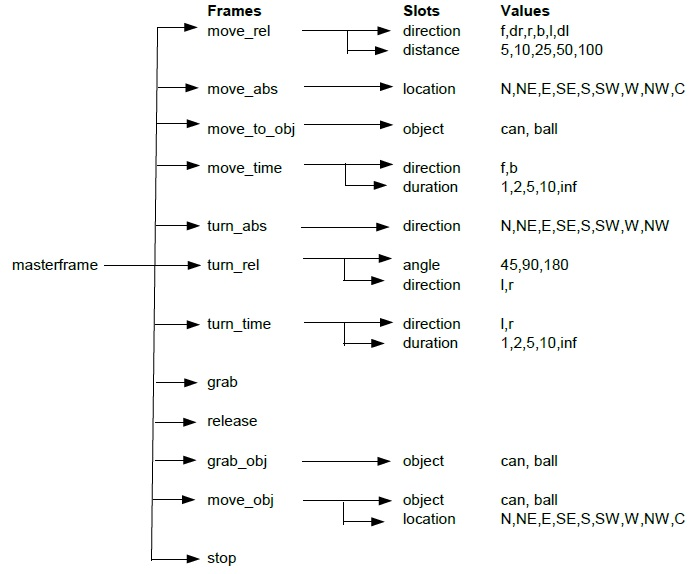
\includegraphics[width=\textwidth]{masterframe.jpg}
\label{masterframe}
\centering
\caption{de masterframe}
\end{figure}
